\documentclass[a4paper,11pt]{memoir} 

\usepackage[utf8]{inputenc}
\usepackage[danish]{babel}
\usepackage[T1]{fontenc}
\usepackage[left=4.0cm, right=2.0cm, top=3.0cm, bottom=3.0cm]{geometry} 
\usepackage{amsmath,amssymb}																						

% SIUnitX  http://ctan.org/pkg/siunitx
\usepackage{siunitx,booktabs}		
\sisetup{per=slash}																						
\sisetup{per-mode = reciprocal}
\sisetup{inter-unit-product = \ensuremath{{}\cdot{}}}
\sisetup{output-decimal-marker = {,} }
\DeclareSIUnit{\kroner}{kr.}

\usepackage{graphicx}
\newsubfloat{figure}% Allow subfloats in figure environment
\usepackage{dcolumn,booktabs}
\usepackage{url}
\usepackage{wrapfig}

% Redigere billed-/tabelteksterne.
\usepackage{caption}
\usepackage{subcaption}
\captionsetup{font=small,
labelfont={it,bf},textfont=sf,
format=hang}

% Packages for color handling
\usepackage[usenames,dvipsnames,svgnames,table]{xcolor}

\usepackage{threeparttable}

\usepackage{lscape}

% TODONotes http://ctan.org/pkg/todonotes
\usepackage{todonotes}
\usepackage{placeins}

\usepackage[hidelinks]{hyperref}  
\hypersetup{bookmarks=false}
\hypersetup{pdftitle={Indlejret digital grafisk equalizer modul}} 
\hypersetup{pdfsubject={4. Semester Projekt, E17, Grp. [3]}}
\hypersetup{pdfauthor={J\"{o}rn Jacobi, Simon Møller, Søren Frank, Kenneth Petersen, Dennis Amtoft Jensen, Jonas Jensen Holmgren}}


% For includering af .pdf
\usepackage{pdfpages}

% Bibliografi
\usepackage{babelbib}
\bibliographystyle{abbrv}

% Noget forsideopsætning
\usepackage{soul} % lege lege
\sodef\an{}{0.2em}{.9em plus.6em}{1em plus.1em minus.1em}
\newcommand\stext[1]{\an{\scshape#1}}

% New commands 
\newcommand{\g}{9,82 \si{\meter\per\second\squared}}
\newcommand{\dcite}[1]{\quotedblbase{#1}\textquotedblright}
\newcommand{\husk}[2]{\todo[inline,color=green!40]{#1: #2}}
\newcommand{\note}[1]{\todo[inline]{#1}}
\DeclareMathOperator{\lapl}{\mathcal{L}}
% Remove paragraph indentation for document
\setlength{\parindent}{0pt}
\newcommand\hcancel[2][black]{\setbox0=\hbox{$#2$}%
	\rlap{\raisebox{.45\ht0}{\textcolor{#1}{\rule{\wd0}{1pt}}}}#2} 

% Listings package
\usepackage{listings}


%Fede overskrifter
\usepackage{kpfonts}
\usepackage{calc}
\setSingleSpace{1.0}
\SingleSpacing
\definecolor{chaptercolor}{gray}{0.8}
% helper macros
\newcommand\numlifter[1]{\raisebox{-2cm}[0pt][0pt]{\smash{#1}}}
\newcommand\numindent{\kern37pt}
\newlength\chaptertitleboxheight
\makechapterstyle{hansen}{
  \renewcommand\printchaptername{\raggedleft}
  \renewcommand\printchapternum{%
    \begingroup%
    \leavevmode%
    \chapnumfont%
    \strut%
    \numlifter{\thechapter}%
    \numindent%
\endgroup%
}
  \renewcommand*{\printchapternonum}{%
    \vphantom{\begingroup%
      \leavevmode%
      \chapnumfont%
      \numlifter{\vphantom{9}}%
      \numindent%
      \endgroup}
    \afterchapternum}
  \setlength\midchapskip{0pt}
  \setlength\beforechapskip{0.5\baselineskip}
  \setlength{\afterchapskip}{1\baselineskip}
  \renewcommand\chapnumfont{%
    \fontsize{3cm}{0cm}%
    \bfseries%
    \sffamily%
    \color{chaptercolor}%
  }
  \renewcommand\chaptitlefont{%
    \normalfont%
    \huge%
    \bfseries%
    \raggedleft%
  }%
  \settototalheight\chaptertitleboxheight{%
    \parbox{\textwidth}{\chaptitlefont \strut bg\\bg\strut}}
  \renewcommand\printchaptertitle[1]{%
    \parbox[t][\chaptertitleboxheight][t]{\textwidth}{%
      %\microtypesetup{protrusion=false}% add this if you use microtype
      \chaptitlefont\strut ##1\strut}%
}}
\chapterstyle{hansen}
\aliaspagestyle{chapter}{empty} % just to save some space

%linje afstand
%\DisemulatePackage{setspace}
%\usepackage[nodisplayskipstretch]{setspace}
%\setstretch{0.5}
%\siglespacing
%\onehalfspacing                                       
%\doublespacing

\usepackage{tikz}
\usepackage{float}
\usepackage{pgfplots}
\usepackage{pgfplotstable}
\pgfplotsset{compat=newest}

\usetikzlibrary{shapes,shadows,arrows}
\newcommand{\dsplinewidth}{0.25mm}           % Line width for connections
\newcommand{\dspblocklinewidth}{0.3mm}       % Line width for blocks
\newcommand{\dspoperatordiameter}{4mm}       % Diameter for adder, multiplier, mixer
\newcommand{\dspoperatorlabelspacing}{2mm}   % Distance from symbol to label for adder, multiplier, mixer
\newcommand{\dspnoderadius}{1mm}             % Filled and empty node
\newcommand{\dspsquareblocksize}{8mm}        % Size for square blocks, e.g. for delay elements, decimator, expander
\newcommand{\dspfilterwidth}{14mm}           % Width of a filter block

\begin{document}
% --------- Frontpage ------------------
\begin{titlingpage}
\thispagestyle{empty}
\centering
{ \setlength{\baselineskip}{24pt}
{\Huge \stext{Indlejret digital parametrisk equalizer modul} \par
%\textit{\&}\par
%\stext{Analogier}
}\par
\stext{Indlejrede systemer og signalbehandling - F17}
\par\vspace*{4\onelineskip}
\par
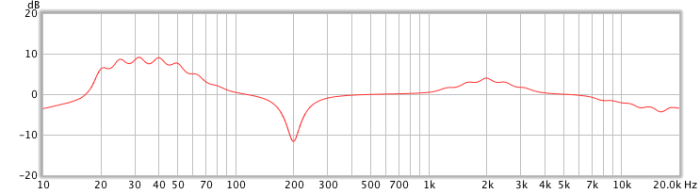
\includegraphics[width=15cm]{billeder/eq-response.png}
\par\vspace*{4\onelineskip}
\stext{4. Semester Projekt}\par

\large\stext{J\"{o}rn Jacobi -- 230674}\par
\large\stext{Simon Juul M\o ller -- 230893}\par
\large\stext{S\o ren Frank -- 300595}\par
\large\stext{Dennis Amtoft Jensen -- 121091}\par
\large\stext{Kenneth Petersen -- 161195}\par
\large\stext{Jonas Jensen Holmgren -- 260785}\par

\vfill
\vspace*{2\onelineskip}
\stext{Gruppe 3}\par
\stext{Vejleder: Steffen Peter Skov }\par
\stext{1. februar - 26. maj 2017}\hfill
%\stext{24. maj 2013}\hfill
\par\vspace*{2\onelineskip}
\small
\stext{M\ae rsk Mc-Kinney M\o ller Instituttet}\par
\stext{Syddansk Universitet}
\enlargethispage{2\onelineskip}
}
\end{titlingpage}


% --------- Abstract -------------------
\newpage
\thispagestyle{empty}
\renewcommand{\abstractnamefont}{\normalfont\bfseries}
\renewcommand{\abstracttextfont}{\normalfont}
\begin{abstract}
I dette projekt designes, realiseres og testes en digital parametrisk equalizer. Equalizeren er designet på baggrund af ... , hvor kravspecifikationenerne er inspireret af allerede markedsførte løsninger.	
\end{abstract}

% --------- Thanks ---------------------
\newpage
\thispagestyle{empty}
\null
\vfill
\begin{center}
\emph{Thanks for all the fish...}
\end{center}

%---------- Underskrift
\newpage
\thispagestyle{empty}
\null

\section*{Underskrifter}
\vspace{3ex} \hfill Underskrevet d. 24/05-2017\\

\newlength{\streg} \setlength{\streg}{0.49\linewidth}
\vspace*{\fill} \rule{\streg}{1pt} \hfill \rule{\streg}{1pt}\\
\begin{minipage}[b]{\streg}
 \centering
 \rule{0pt}{4ex}
 J\"{o}rn Jacobi \\
 {\footnotesize (230674) (jojac11@student.sdu.dk)}
\end{minipage}
\hfill
\begin{minipage}[b]{\streg}
 \centering
 Simon Møller \\
 {\footnotesize (230893) (simmo03@student.sdu.dk)}
\end{minipage}

\vspace*{\fill} \rule{\streg}{1pt} \hfill \rule{\streg}{1pt}\\
\begin{minipage}[b]{\streg}
 \centering
 \rule{0pt}{4ex}
 Søren Frank \\
 {\footnotesize (300595) (sofra15@student.sdu.dk)}
\end{minipage}
\hfill
\begin{minipage}[b]{\streg}
 \centering
 Dennis Amtoft Jensen \\
 {\footnotesize (121091) (dejen14@student.sdu.dk)}
\end{minipage}

\vspace*{\fill} \rule{\streg}{1pt} \hfill \rule{\streg}{1pt}\\
\begin{minipage}[b]{\streg}
	\centering
	\rule{0pt}{4ex}
	Kenneth Petersen \\
	{\footnotesize (161195) (kepet15@student.sdu.dk)}
\end{minipage}
\hfill
\begin{minipage}[b]{\streg}
	\centering
	Jonas Jensen Holmgren  \\
	{\footnotesize (260785) (jonho12@student.sdu.dk)}
\end{minipage}	

\newpage
\thispagestyle{empty}
\null
\vfill

%---------- Forord
\newpage
\thispagestyle{empty}
\chapter*{Forord}\label{chap:forord}
\addcontentsline{toc}{chapter}{Forord}

Dette projekt er udarbejdet af studerende på 4. semester elektronik og datateknik, ved Syddansk Universitet, Teknisk Fakultet, foråret 2017. Projektet er en sammenfatning af de opnåede fagligheder fra semesterets undervisning. Afleveringen af rapporten er dertil et krav for at kunne gå til eksamen.

\jj{Beskrive hvem vi forventer at læseren er til}

\subsection{Læsevejledning}
Denne rapport er opbygget således, at den læses fra start til slut. Rapportens struktur er opdelt i hovedsektioner og undersektioner. Opbygningen er taksonomisk både i kapitelstrukturer og som helhed. Der vil i starten af hvert hovedafsnit være en figur som viser hvilken del af produktet der i det respektive afsnit bliver dækket.

\subsection{Typografiske konventioner}
Her er en kort oversigt over de typografiske konventioner der anvende i denne rapport
\\
\textit{Kursiv tekst} : Angiver filnavne i den tilhørende kodebase.
\\
\textbf{Fed tekst} : Bruges til a fremhæve produkt eller system specifikke betegnelser.
\\
\texttt{Konstant brede tekst} : Anvendes til kildekode eksempler.
\\
\emph{Fremhævet tekst} : Bliver brugt når der gives en kort introduktion til hvert kapitel. 
\\
\jj{Gennemgang af alle typografier og at de bliver brugt rigtigt igennem rapporten.}

\husk{Kenneth}{Noget med arbejdsfordelingen}

\note{Hvem har skrevet (og evt. udgivet) rapporten - og hvornår?
	Hvorfor er den blevet skrevet - hvad er dens baggrund, og hvem er dens målgruppe?
	Hvordan er den blevet til? (Yderst kort: arbejdsmetodik, afgrænsning, evt. projektperiode)
	Hvad er formålet med rapporten? Hvem er den skrevet til gavn for, og hvad skal de kunne bruge den til?
	Eventuel tak til vejledere, faglige hjælpere, økonomiske bidragydere osv.}

\note{Forordet skal handle om selve rapporten. Det skal give læseren et billede af, hvad det egentlig er for et værk, han eller hun sidder med:}


\newpage
\thispagestyle{empty}
\null
\vfill

%---------- Indholdsfortegnelse  ---
\newpage
\tableofcontents*												
\newpage

\DoubleSpacing	
%---------- Kalibrerings side --------
%Lorem ipsum dolor sit amet, pri ipsum partiendo interpretaris ea. Eum meliore persecuti no, at fugit quando mei. Nibh aliquid cum ei. Ne utinam libris nec, ex aliquip antiopam pri. Nam assum affert ancillae an, eos ea hinc mundi, dolor eleifend volutpat no usu. Ut nam esse essent ponderum. Ut eam quidam partiendo deterruisset, te pri consequuntur concludaturque. In oportere abhorreant vis, in usu ludus graeco volutpat, vel iudico dicunt prodesset ea. Mei natum noster eu, mei no ornatus ocurreret.
Pri unum maiestatis in, agam audiam perfecto ne mel. Ut per invenire petentium adolescens. An mei propriae phaedrum postulant. Vim amet electram ei. Ea wisi dolorem qui, mea propriae persecuti ad, option nusquam nominati ut mei. Nam te animal inermis, verear neglegentur ius id. His quem prompta inermis id, eruditi invidunt vix id. Eu sea tota vidisse deseruisse, aliquid nostrum voluptua ea vel. Facete audiam abhorreant an eum. Vim magna appellantur ne, vidit nulla sed ut. Mei nostrum vituperata consectetuer no. Noluisse placerat salutandi qui eu. Cum eu illud clita. Est vivendum convenire ex, sit primis iriure neglegentur an, ex sed modus tincidunt. Evertitur pertinacia constituam eu mea. Oblique alienum ocurreret ius ad. In eos aeterno iuvaret liberavisse, accusata euripidis an per. Nibh detracto placerat sea ut. Pri an minim aperiam omnesque, ancillae appareat reformidans ius in. Cibo aeterno erroribus ut eam, vim recteque scribentur liberavisse eu, choro soluta dolorem vis ea. Ad vel nullam graece legendos, sit melius menandri expetenda at. Sea inermis dolores ad, ut has noster argumentum. Qui movet zril an, in nam nobis quando. Usu ne saperet nostrum, per te nominati accusamus sententiae, est cu debet virtute accusata. Nihil fastidii his cu, pri aeterno persius vivendo id. Per te wisi temporibus, ullum iudicabit mea te, duis recusabo ea vel. Vim quodsi accumsan ut, te pro explicari iracundia. Vim id molestiae posidonium, clita everti facilisis ius te. Cu adhuc convenire comprehensam vis, decore facilis torquatos qui ne, at qui duis legendos sarium.
Zril commodo theophrastus cu cum. Eu reformidans conclusionemque sit, vix eu cibo everti similique, ex duo munere omnium principes. An vel sapientem moderatius, malis lobortis partiendo vel ne. Ea quod graeci expetenda usu.
Denne tekst er skrevet med Century Schoolbook fontstørrelse 11, med en afstand på 8pkt. efter afsnit og linjeafstand på 1.5.
%\newpage

%---------- Indledning -------------
\chapter{Indledning}
\vspace*{0.5 cm}
\emph{Musik er en naturlig del af hverdagen. 
	Om det er baggrundsmusikken nede i Brugsen, en Grøn Koncert eller i høretelefonerne i bussen, er den altid til stede. 
	At musikken er så væsentlig en størrelse giver anledning til at undersøge hvilke optimeringsmåder man kan foretage sig, for at få den bedst mulige oplevelse ud af det - hver især. 
	En equalizers egenskab er at forme en musikafspillers lydsignal, så musikken lyder som brugeren finder bedst. 
	I denne rapport vil læseren blive guidet gennem processen bag ved udvikling af en digital equalizer - fra musikafspillerens udgangssignal til det ønskede lydsignal.}

\section{Formål}
%\note{Indledningen skal ikke handle om rapporten, men om rapportens emne. Man kan sige, at den kridter banen op ved at præsentere emneområdet.
%	\\
%	* Hvilket overordnet emne tager rapporten udgangspunkt i? \\
%	* Hvilket specifikt problem vil man derfor tage fat i og kigge nærmere på? }
%
%Formålet med projektet er, at forene de opnåede fagligheder fra undervisningen, samt at træne den studerende i, at kunne forstå og forklare afgrænsede systemer med funktionalitet der relaterer til faglighederne i Indlejrede Systemer og Signalbehandling, på 4. semester Elektronik og Datateknik. Fagene fra semesteret der indgår i projektet er Embedded programmering, Analoge filtre og signaler og Operativsystemer. Ledningsteori som er et mindre fag under Analoge filtre, er ikke med i rapporten, da undervisningen ligger så sent i semesteret, at der ikke er tid til at se på implementation af faget i rapporten.
%
%Semesterets fagbeskrivelse vil blive brugt som tjekliste, for at komme igennem så meget af stoffet som muligt.
Formålet med dette projekt, er at formidle de opnåede fagligheder fra 4. semesters undervisning på uddannelsen diplomingeniør i elektronik og datateknik. Semesterets hovedemne omhandler "Indlejrede systemer og signalbehandling", hvor fagene "Analoge filtre og signaler", "Digital signalbehandling", "Embedded programmering" og "Operativsystemer" er inkluderet. Der skal på et grundlæggende niveau, kunne relateres til faglighederne i ét samlet produkt ud fra disse. For at kunne håndtere dette, vil semesterets fagbeskrivelse blive anvendt til at opnå det ønskede formål.


\section{Problemformulering}
%\note{Generel fortælling om hvordan man kan finde frem til en projekt der kan blive dækket af de fagligheder de skal omhandle}
%
%\note{Specefike problemer der kan være ved at lave en equalzier som et embedded system}
%
%\note{Hvilke spørgsmål kan der stilles om man ønsker at få besvaret ?}

%Ud fra formålet med projektet, er der blevet valgt, at udvikle en digital equalizer, da den dækker centrale punkter af fagbeskrivelsen. De væsentligste punkter som projektet dækker er analog og digital filterteori, signalbehandling og strukturelle opbygning af et operativ system.

%\note{Problemformulering: Hvilket spørgsmål vil denne rapport helt præcist stille skarpt på, og hvilke delspørgsmål vil det måske være nødvendigt at besvare for at kunne besvare hovedspørgsmålet?}
%
%Hovedspørgsmålet som der vil blive fokuseret på er:
%\begin{enumerate}
%	\item Hvilken digital signalbehandling kan give den ønskede signal filtrering?
%\end{enumerate}
%Herunder ses underspørgsmålene som vil blive brugt til at besvare hovedspørgsmålet:
%\begin{enumerate}
%	\item Kan en digital equalizer realiseres ved hjælp af en Tiva™ TM4C123GH6PM Microcontroller?
%	\item Kan EMP boarded fra Embedded Programmering anvendes i projektet?
%	\item 
%\end{enumerate}
%\note{
%Projektet går ud på at designe en parametrisk equalizer, der kan efterbehandle et lydsignal. Den skal realiseres ved hjælp af en Tiva™ TM4C123GH6PM Microcontroller som er platformen i faget Embedded Programmering. Equalizeren skal have nogle forudbestemte bånd, og samtidig have et bånd som brugeren frit kan modulere.
%}
Ud fra formålet for projektet, er der blevet valgt at fremstille et produkt, hvori alle fagligheder kan anvendes. 
Produktet der ønskes realiseret, er konstruktionen af en digital parametrisk\footnote{Uddybende forklaring om forskellen mellem parametrisk og grafisk equalizer findes i kapitel \ref{kap:equalizer}.} equalizer. 
Denne parametriske equalizer, skal realiseres ved en mikrocontroller af samme type, der anvendes som platformen i faget "Embedded programmering".
Equalizeren skal have nogle såkaldte "bånd" med justerbare parametre, som fx frekvens og forstærkning. 
Ud fra fagbeskrivelsen, kan dette relateres i et så bredt omfang, at formålet opfyldes. 
Problemformuleringen forlyder sig derfor som følgende: \\

En digital parametrisk equalizer ønskes realiseret ved en mikrocontroller hvor der anvendes digital signalbehandling og analog filterteori. 
Herunder ønskes en brugerflade, som interagerer med systemet. 
Denne brugerflade skal kunne håndtere equalizerens båndprofiler.\\

Der ønskes herudover svar på følgende problemstillinger.
\begin{itemize}[noitemsep]
	\item Hvilke digitale signalbehandlingsmetoder er egnet til fremstilling af en digital equalizer?
	\item Hvordan anvendes digital signalbehandling, til at give de ønskede båndspecifikationer?
	\item Hvordan anvendes analoge filtre i en digital equalizer?
	\item Hvilke krav er der til de analoge filtre i forhold til den samlede signalbehandling.
	\item Hvordan fremstilles og designes software der kan håndtere digital sampling og gengivelse af lydsignalet
\end{itemize}

\section{Projektafgrænsning}
%\note{Hvilke emner / delemner kommer rapporten ikke ind på? Hvorfor?\\
	%Det er meget almindeligt, at problemformulering og metoderedegørelse simpelthen er en del af indledningen, men så bør de normalt være markeret med underrubrikker (under-overskrifter) for overskuelighedens skyld. Hvis du er uddannelsessøgende, så tjek, om skolen eller institutionen (eller din vejleder) har særlige krav på det punkt.}

En equalizer kan realiseres både analogt og digitalt.
I projektet vil den blive realiseret digitalt, da faget "Embedded programmering" skal indgå. 
Der træffes endvidere valget om at gøre den parametrisk, for bedre fleksibilitet. 
Følgende medtages ikke i rapporten og afgrænser projektet:
\begin{itemize}[noitemsep]
	\item Equalizeren bliver udviklet som prototype og ikke et produktionsklart produkt.
	\item Der vil blive lagt vægt på at eftervise funktionaliteten af signalbehandlingen og ikke hvor god lydkvalitet det endelige produkt lever op til.
	\item Koden som er anvendt til equalizeren, er så vidt muligt af eget design. Enkelte steder er kode fra 3. part anvendt, herunder moduler og kode eksempler fra undervisningen.
\end{itemize}

\section{Kravspecifikation} \label{afs:kravspecifikation}
I dette afsnit fremstår de opsatte krav for projektet.
Disse er fastsat dels ud fra kravet til selve projektbeskrivelsen og dels for at efterligne den virkelige ingeniørverden.

\begin{itemize}[noitemsep]
	\item Prototypen udvikles på Tiva™ C Series TM4C123G LaunchPad Evaluation Kit \cite{spmt281a}.
	\item Tiva™ TM4C123G serie Microcontroller anvendes \cite{spmu296}.
	\item Kildekoden er en del af produktet og skal overholde \textit{EMP C Code Standard}\cite{emp-c}.
	\item Equalizeren skal fungere som parametrisk equalizer.
	\item Det skal være muligt at ændre frekvensprofiler på equalizeren.
	\item Indgangs- og udgangssignaler skal overholde line-signal standard på, nominal $-10 dBV$, $0,894 V_{pp}$ (Forbruger elektronik line-signal).
	\item Tilgængelige filtertyper i frekvensprofiler - Highshelf, Lowshelf, Peak- og Notchfilter.
	\item Equalizerparametre skal omfatte - Frekvens, båndbredde og forstærkning.
	\item Equalizerens funktionalitet og effektivitet skal kunne efterprøves.
\end{itemize}


\section{Løsningsmodel}

\begin{figure}[h]
	\centering
	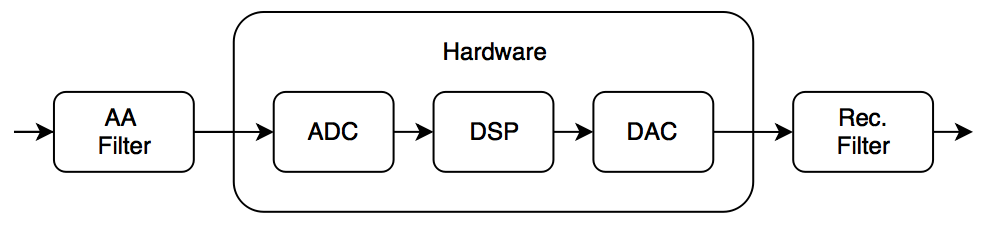
\includegraphics[width=0.8\linewidth]{billeder/flow_losn}
	\caption{Løsningsmodellen}
	\label{fig:losningsmodel}
\end{figure}

Løsningsmodellen som ses på figur \ref{fig:losningsmodel}, er delt op i tre hovedemner. Denne model gør det nemt at dele emnerne som indgår i rapporten op. Figuren kan ses i starten af hvert hovedkapitel, så man nemt kan danne et overblik over hvilken del der tages hånd om. Som første emne er der filtrene - altså både indgangs- og udgangsfiltret. Efter indgangsfiltret går man ind i hardware-blokken, som blandt andet indeholder den analoge til digitale konverter samt den digitale til analoge konverter. Til sidst er der emnet som indeholder den digitale signalbehandling, hvor de matematiske udregninger samt implementering af signalbehandling bliver dækket. 


\section{Proces- og arbejdsmetode}
%\note{Metodebeskrivelse: Hvordan vil det blive gjort? (Opgaven bygger på den-og-den litteratur samt interviews med dem og dem. Først undersøger vi dét, og så undersøger vi dét. Derefter …)}
Denne rapport er bygget op på baggrund af den faglige undervisning, hvor alle fag har spillet en væsentlig rolle. Dertilhørende litteratur er brugt til at studere nærmere specifikke omstændigheder, og ekspertviden er blevet hentet fra underviserne, med bedre forståelse for det faglige indhold. Der er arbejdet ud fra emneopdeling, hvor gruppen er blevet delt i 3, og har fået tildelt arbejdsopgaver ud fra dette. Der er så vidt muligt holdt statusmøder, hvor gruppen har diskuteret hver deres problemer. Der er derudover fulgt en overordnet tidsplan, hvor enkelte deadlines har været opretholdt. Der har været en del miskommunikation imellem gruppen igennem projektperioden, hvilket har gjort at tidsplan mm. har skredet. Der blev dog fundet en fornuftig løsning i samarbejde med gruppens vejleder.

%Gennemarbejdningen med denne rapport vil tage udgangspunkt i undervisningen med dertilhørende litteratur. Ekspertviden vil blive hentet fra underviserne, med henblik på bedre forståelse af stoffet. Rapporten er bygget op omkring signalvejen igennem equalizeren. Det kan derved lette forståelsen for, hvordan signalet ændres løbende igennem systemet.
%\husk{Kenneth}{Tage udgangspunkt i signalvejen - men bedre ord for det}


							

\listoftodos
%\newpage
\section{How To do stuff in LaTeX}

\subsection*{Figur, enkelt}
%-----------------------------------------------------------------------------
\begin{figure}[h!]
	\centering
		\includegraphics[width=.5\textwidth]{billeder/sample.png}
	\caption{Her skrives en god caption til figuren.}
	\label{fig:sample_fig_ref_her}
\end{figure}
\FloatBlock
%-----------------------------------------------------------------------------

\subsection*{Figur, dobbelt}
%-----------------------------------------------------------------------------
\begin{figure}
	\centering
	\subbottom[]{%
  		\includegraphics[width=.39\textwidth]{billeder/sample.png}
	  	\label{fig:sample_fig_ref_her_a}}
	\subbottom[]{%
		\includegraphics[width=.39\textwidth]{billeder/sample.png}
		\label{fig:sample_fig_ref_her_b}}
  	\caption{Her skrives en god caption til figuren.}
	\label{fig:sample_fig_ref_her_samlet}
\end{figure}
\FloatBlock
%-----------------------------------------------------------------------------

\subsection*{Kommentar}
%-----------------------------------------------------------------------------
\husk{Initialer}{Kommentaren skrives her}
%-----------------------------------------------------------------------------

\subsection*{Math Simple}
%-----------------------------------------------------------------------------
\begin{align}
D = \frac{1}{\Delta F}
\end{align}
%-----------------------------------------------------------------------------

\subsection*{Math uden nummer og align}
%-----------------------------------------------------------------------------
\begin{align}
D &= \frac{1}{\Delta F} \Rightarrow \nonumber \\
\Omega &= \mathrm{Noget helt andet}
\end{align}
%-----------------------------------------------------------------------------
\subsection*{Tabeller med caption}
\begin{table}
\centering
    \caption{Konstanter som bruges i overstående formler.}
\label{tab:konst1}
    \begin{tabular}{ | l | l |}
    \hline
    A & 18 [V] \\ \hline
    f & 50 [Hz]  \\ \hline
    T & 20 [s]  \\ \hline
    $\omega$ & 30 \\ \hline
    k & 100 \\ \hline
    \end{tabular}
    \end{table}

\newpage

%---------- Chapter ----------------
\chapter{Chapter}\label{kap:chap1}



Dette kapitel omhandler definition af equalizer, forskellige typer
og dets brugbarhed indenfor lyd, herunder også kravspecifikationer.


%---------- Parts ----------------
\section{Section}\label{sec:sect1}

%---------- Chapter ----------------
\chapter{Digitale filtre og signalbehandling}\label{kap:filter}

\begin{figure}[h]
	\vspace*{-1 cm}
	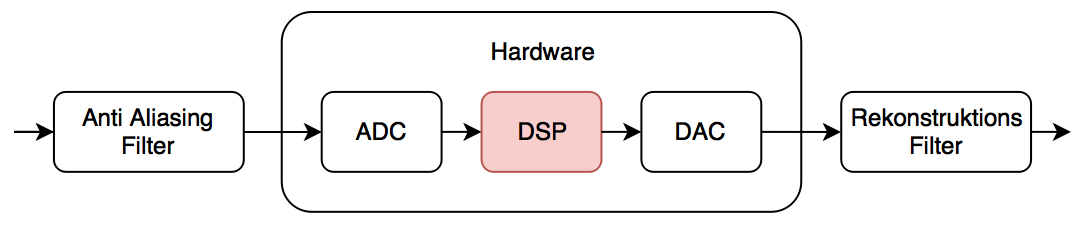
\includegraphics[width=8cm]{billeder/flow_dsp}
	\vspace{0.5 cm}
\end{figure}

\emph{I dette afsnit vil teorien bag IIR og FIR filtrene blive gennemgået, hvoraf det ene filter vil blive realiseret i praksis.}

%---------- Parts ----------------
\section{FIR - Finite Impulse Response}\label{sec:fir}
Formålet med FIR filteret er at udregne filter koefficienterne, $b_{i}$, der bruges til at approksimere størrelsen af frekvens responset af FIR filteret, $H(z)$.
\Kenneth{\cite[Side. 217]{}.}
Forholdet mellem input og output (også kaldet differensligning) i et kaulsalt FIR filter er givet ved ligning \ref{fir_ligning},
\begin {equation} 
y(n)=\sum\limits_{i=0}^{K}b_{i}x(n-i) \label{fir_ligning}
\end {equation}
hvor $b_{i}$ repræsenterer filterets koefficienter og $K+1$ er filterets længde. Nuværende og tidligere sampleværdier bliver brugt til at beregne den næste output sample, og det har den fordel, at filtreringen kan ske i real-tid.
\\
\Kenneth{\cite[Side. 218]{}.}
Derefter z-transformeres ligning \ref{fir_ligning}. For at opskrive FIR filterets overføringsfunktion, faktoriseres $X(z)$ ud på højre side af den z-transformerede ligning \ref{fir_ligning} og derefter dividere igennem med $X(z)$ fås ligning \ref{fir_transfer}.
\Kenneth{Overføringsfunktion}
\begin {equation}
H(z)=\frac{Y(z)}{X(z)}=b_{0}+b_{1}z^{-1}+...+b_{K}^{-1} \label{fir_transfer}
\end {equation}

Input og output signalet er givet ved foldning og er opskrevet i ligning,
\Kenneth{Ved ikke om den skal med?}
\begin {equation} 
\sum\limits_{i=0}^{N-1} h(k)x(n-k) 
\end {equation}
hvor $h(k)$ er impulsresponset. Modsat IIR filterne, har FIR en endelig længde, $N$, antal værdier. FIR filterets impulsrespons er et sæt af filter koefficienter. Sendes en impuls ind i filteret bestående af et $"1"$ efterfulgt af mange $"0"$er, bliver filterets output det sæt af koefficienter $"1"$-samplen kører igennem. 


FIR filterets overføringsfunktion er givet ved ligning \ref{FIR_transfer}

\begin {equation}
H(z)=\sum\limits_{k=0}^{N-1}h(k)z^{-1} \label{FIR_transfer}
\end {equation}

\section{Design metoder} \label{sec:fir_design}
Herunder redegøres der for 2 forskellíge design metoder, til beregning af filter koefficienter.
\subsection{Frekvenssampling}
Ved frekvenssampling approksimeres det ønskede frekvensrespons ved, at sample det $N$ antal gange, med samme interval imellem samplingspunkterne. Der kan derved opnås et interpolateret frekvens respons.
Pointen med frekvenssampling er at filterkoefficienter kan beregnes udfra specificerede størrelser i forhold det ønskede filter respons uniformt i frekvensdomænet.

Filterkoefficienterne kan beregnes udfra definitionen af den inverse DFT (IDFT):
\Kenneth{\cite[Side. 262]{}.}
\begin {equation}
h(n)=\frac{1}{N}\sum_{k=0}^{N-1}H_{d}(k)W_{N}^{-kn} ,\hspace{1cm}\text{for}\hspace{1cm} n = 0, 1,\text{ ... }, N-1 \label{fir_filterkoefficienter}
\end {equation}
hvor
\begin {equation}
W_{N}=e^{j\frac{2\pi}{N}} \hspace{1cm}\text{og} \hspace{1cm} H_{d}(k)=h(e^{j\Omega_{k}}) \nonumber
\end {equation}
Der antages lineær fase og at antallet af samplingspunkt er $N=2M+1$.



\begin{figure}[h]
\centering
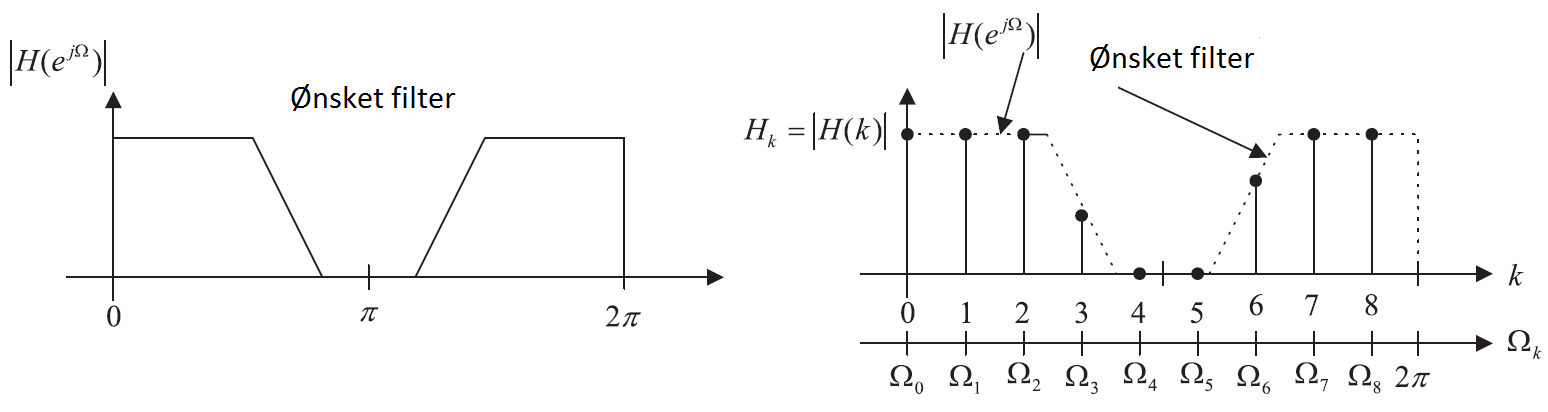
\includegraphics[width=.90\textwidth]{billeder/fir_frekvenssampling.png}\label{fig:fir_frekvenssampling}
\caption{Ønskede filterrespons og samplede filterrespons.}
\end{figure}
\FloatBlock

Ligning \ref{fir_filterkoefficienter} kan simplificeres til,
\begin {equation}
h(n)=\frac{1}{2M+1}\left[ H_{0}+2\sum_{k=1}^{M} \left( \frac{2\pi k(n-M)}{2M+1} \right) \right] \hspace{1cm} \text{for} \hspace{1 cm} n=0,1,\text{ ... },2M
\end {equation}

hvor $h(k)$ for $k=0,1,\text{ ... },2M$, repræsenterer filterkoefficienternes størrelser, der bruges til at specificere det ønskede filterrespons med samplingslængden $\Omega_{k}=\frac{2\pi k}{(2M+1)}$.

Design proceduren opskrives:
\Kenneth{\cite[Side. 263]{}.}
\\
\begin{enumerate}[noitemsep,nolistsep]
\item Ud fra filterlængden $2M+1$, angives størrelsen af frekvensresponset for det normaliserede filter gående fra $0$ til $\pi$.
\begin{equation}
	H_k \text{ ved } \Omega_{k} = \frac{2 \pi k}{2M+1} \hspace{1cm} \text{for} \hspace{1cm} k=0,1,\text{ ... , } M
\end{equation}
\item Udregn FIR koefficienterne
\begin{equation}
b_n = h(n)=\frac{1}{2M+1}\left[ H_{0}+2\sum_{k=1}^{M} \left( \frac{2\pi k(n-M)}{2M+1} \right) \right] \hspace{1cm} \text{for} \hspace{1 cm} n=0,1,\text{ ... },2M
\end{equation}
\item Anvend symmetri (heraf krav om lineær fase) til at finde resten af keofficienterne.
\begin{equation}
	h(n) = h(2M-n) \hspace{1cm} \text{for} \hspace{1cm} n=M+1 \text{, ..., } 2M
\end{equation}
\end{enumerate}

\subsection{Windowsmetoden}
Den grundlæggende tilgang til windowsmetoden er baseret på at det ideelle lavpas-, højpas-, båndpas-, og båndstop filter, bestående af den følgende ikke-kausale impulsrespons på $-\infty < n < \infty$. Windowsmetoden bygger på Fourier Transformationen, hvor det gælder om at fjerne de uønskede Gibbs oscilleringer i pas- og stopbåndet, som finder sted under trunkeringen. Anvendes windowsmetoden på filterkoefficienterne fås ligning \ref{window_function},
\Kenneth{\cite[Side. 230]{}.}
\begin{equation}
	h_w(n) = h(n)*w(n) \hspace{1cm}\text{,} \hspace{1cm}n=-M,\text{ ... },0, 1,\text{ ... , }M	
	\label{window_function}
\end{equation}
hvor $w(n)$ angiver det valgte vindue.

For at beregne koefficienterne for $h_w$, forsinkes impuls sekvensen med M samples som ses i ligning \ref{b_n-window}
\begin{equation}
	b_n = h_w (n-M), \hspace{1cm} \text{for} \hspace{1cm} n = 0,1, \text{ ... , }M \label{b_n-window} 
\end{equation}

Grundlaget for valg af vindue baseres blandt andet på overgangsbåndet $\Delta f$.

\begin{equation}
\Delta f = \frac{f_{stop}-f_{pas}}{f_s} \label{Windows_transistionband}
\end{equation}

Ripplen i henholdsvis pas- og stopbåndet beregnes udfra ligning \ref{ripple_p} og \ref{ripple_s}.

\begin{align}
\delta_p dB &= 20*log_{10}(1+\delta_p) \label{ripple_p}\\
\delta_s dB &= -20*log_{10}(\delta_s) \label{ripple_s}
\end{align}

Filterets knækfrekvens, $f_c$, bestemmes ud fra midten af overgangsbåndet. En tommmelfingerregel til bestemmelse af $f_c$ er givet ved ligning \ref{fir_cutoff}
\Kenneth{\cite[Side. 241]{}.}
\begin{equation}
	f_c =\frac{f_{pas}-f_{stop}}{2} \label{fir_cutoff}
\end{equation}

%\begin{equation}
%h_{d,LP}[n] = \frac{sin(\omega_c n)}{\pi n} \label{windows_lp}
%\end{equation}
%\begin{equation}
%h_{d,HP}[n] = \delta(n) - \frac{sin(\omega_c n)}{\pi n} \label{windows_hp}
%\end{equation}
%\begin{equation}
%h_{d,BP}[n] = \frac{sin(\omega_b n) - sin(\omega_a n)}{\pi n} \label{windows_bp}
%\end{equation}
%\begin{equation}
%h_{d,BS}[n] = \delta(n) - \frac{sin(\omega_b n) - sin(\omega_a n)}{\pi n} \label{windows_bs}
%\end{equation}

%Ligningerne \ref{windows_lp}, \ref{windows_hp}, \ref{windows_bp} og \ref{windows_bs} er de generelle filterfunktioner. 
Efter valget af hvilken filtertype der skal anvendes, findes det nødvendige vindue, at påtrykke filteret med.

Fremgangsmetoden for windowsmetoden ses i de følgende 5 trin:
\begin{enumerate}[noitemsep,nolistsep]
	\item Ud fra de ønskede filterspecifikationer, bestemmes filterordenen og knækfrekvensen. Der vælges en vinduesfunktion og ligning \ref{fir_cutoff} anvendes.
	\item Beregn impulssekvensen $h(n)$ ved hjælp af Fourier transformations metoden.
	\item Multiplicer det genererede filter koefficienter $h(n)$ i trin 2 med det valgte vindue, for at at opnå impulssekvensen for vinduet $h_w(n)$.
	\item Forsink vinduesimpulsen $h_w(n)$ med M samples for at få det kausale filters koefficienterne $b_n = h_w(n-M)$ med ligning \ref{b_n-window}.
	\item Overføringsfunktionen plottes, og hvis kravene til frekvensspecifikationer ikke er opfyldt, øges filterets orden og proceduren gentages.
\end{enumerate}

%---------- Chapter ----------------

%---------- Parts ----------------

%---------- Chapter ----------------

%---------- Parts ----------------


%---------- Chapter ----------------

\chapter{Diskussion og vurdering}\label{kap:diskussion}
\emph{I dette kapitel vil udvalgte elementer i rapporten blive diskuteret}

\subsection{Analoge filtre}

\subsection{Hardware og operativ system}

\subsection{Digital signalbehandling}

\begin{itemize}
\item Fixed point beregning.
\item Assembler optimerede funktioner.
\end{itemize}
\subsection{Equalizer test}
							

%---------- Chapter ----------------
\chapter{Konklusion} \label{kap:konklusion}
\Kenneth{Opdele en konklusion fra hvert kapitel.
	Måske også en perspektivering}

Hvad var muligt, og hvad viste sig at være for omfattende til tidshorisonten?

Ting der skal besvares fra problemformuleringen. Rækkefølge endnu uvist.
\begin{itemize}[noitemsep]
	\item Hvilke digitale signalbehandlingsmetoder er bedst til fremstilling af en digital equalizer?
	\item Hvordan kan et analogt filter anvendes på en digital equalizer?
	\item Hvordan anvendes digital signalbehandling, til at give de ønskede båndspecifikationer?
	\item Hvilke krav er der til de analoge filtre i forhold til den samlede signalbehandling.
	\item Hvordan fremstilles og designes software der kan håndtere digital sampling og gengivelse af lydsignalet
\end{itemize}							


\SingleSpacing

\nocite{*}
\bibliography{rapport}\label{bilag:litteratur}
%\listoffigures
%\listoftables

%--------- Bilag -------------------
\appendix
%\chapter{Ordliste} \label{bilag:ordliste}

\begin{table}[h!]
	\caption{Ordliste}
	\label{tab:ordliste}
	\begin{threeparttable}
		\begin{tabular}{l p{0.7\textwidth}}
			\toprule
			\textbf{Ord}      & \textbf{Beskrivelse}   \\ 
			\midrule
			ADC			& Analog digital converter (Eng.)\\
			ANSI		& American National Standards Institute (Eng.)\\
			API			& Grænseflade på en computer der tillader én softwarekomponent at kommunikere med en anden\tnote{a}\\
			CLI			& Commandline interface (Eng.)\\
			DAC			& Digital analog converter (Eng.)\\
			Equalizer 	& Elektronisk apparat eller komponent som i forbindelse med forstærkning af lyd regulerer forholdet mellem de forskellige frekvensers styrke for at opnå en bedre klang \tnote{a} \\
			Latency		& (Eng.) Tidsforsinkelsen imellem stimulans og respons.\\ 
			LCD			& Liquid crystal display (Eng.) \\
			MCU       	& Micro Controller Unit (Eng.). Microcontroller eller mikroprocessor. \\
			Monotonic 	& (Eng.) En evig stribe af små gentagelse.  \tnote{a}\\
			Periferienhed & Selvkørende hardwaremodul i mikrocontrollerens arkitektur.\\
			Preemptive	& (Eng.) Afbrydelse af task fra fx. en scheduler.\\
			PWM			& Pulse Width Modulation (Eng.) \\
			SAR			& Successive Approximation Register (Eng.)\\
			Shell		& Brugerinterface (CLI) til operativsystemets funktionalitet.\\
			SPI			& Serial Peripheral Interface (Eng.)  \\
			UART		& Universal asynchronous receiver and transmitter (Eng.)\\
			\bottomrule
		\end{tabular}
	
		\begin{tablenotes}
			\item[a] \textit{Den Danske Ordbog - \url{http://ordnet.dk/}}
		\end{tablenotes}
	\end{threeparttable}
\end{table}

\chapter{Bilag}
%\chapter{Symbolforklaring} \label{bilag:symbol}

\begin{table}[h!]
\centering
\caption{Symbolforklaring}
\label{tab:symboler}
\begin{threeparttable}
\begin{tabular}{l l l}
\toprule
\multicolumn{1}{l}{Symbol}       &
\multicolumn{1}{l}{Enhed}        &
\multicolumn{1}{l}{Beskrivelse}  \\ 
\midrule
$A_{ki}$\tnote{*}	    &   			& Matrice af $K$ 2. ordens filters nævner polynomie.\\
$a_i$\tnote{*}	    &   				& Nævner polynomie af overførings funktion.\\
$B_{ki}$\tnote{*}	    &   			& Matrice af $K$ 2. ordens filters tæller polynomie.\\
$b_i$ \tnote{*}	    &   				& Tæller polynomie af overføringsfunktion.\\
$C$ & [\si{\farad}] & Elektrisk kapacitans \\
$E_T$ & [\si{\volt}] & Ikke korrigerede maksimal fejl i ADC. \\
$F_{CPU}$ & [\si{\hertz}] & CPU'ens clockfrekvens. \\
$F_{SCK}$ & [\si{\hertz}] & SPI clockfrekvens.\\
$f$					&	[\si{\hertz}]	& Frekvens.	\\
$f_0$				&	[\si{\hertz}]	& Centerfrekvens.	\\
$f_c$				&	[\si{\hertz}]	& Knækfrekvens.	\\
$f_s$				&	[\si{\hertz}]	& Samplingsfrekvens.	\\
$G$\tnote{*}		&   				& Forstærkning. Kan beskrives i [\si{\decibel}].\\
$G_0$\tnote{*}		&   				& Reference forstærkning. Kan beskrives i [\si{\decibel}].\\
$G_B,G_C$\tnote{*}	&   				& Forstærkning ved knækfrekvens. Kan beskrives i [\si{\decibel}].\\
$H(s)$\tnote{*}	    &		            & Overføringsfunktion i s-domænet.	\\
$H(z)$\tnote{*}	    &		            & Overføringsfunktion i z-domænet.	\\
$|H|$\tnote{*}	    &		            & Amplitude af overføringsfunktion.	\\
$\Im$\tnote{*}		&					& Imaginærdelen af et complex tal.	\\
$i$\tnote{*}		&					& $\sqrt{-1}$ imaginær tal.	\\
$K$ & & Filter længde\\
$M$\tnote{*}        &                   & Antal samples \\ 
$N$\tnote{*}        &                   & Filters orden.\\
$N_{CPU,cycles}$ & & Antal cycles per sample \\
$N_{kanal}$\tnote{*} & & Antal kanaler. \\
$Q$\tnote{*}        &                   & Filtres godhed.\\
$R$ & [\si{\ohm}] & Elektrisk resistans \\
$\Re$\tnote{*}		&					& Realdelen af et complex tal.	\\
$s$\tnote{*}		&					& Variable til laplace-transformeret overføringsfunktioner.\\
$T_C$ &[\si{\second}] & ADC's sampletid. \\
$T_s$ & [\si{\second}] & Samplingstid. \\
$t_{cmd}$ & [\si{\second}] & Transmissions tid af SPI kommando for DAC.\\
$t_{setling}$ &[\si{\second}] & Indsvingningstid. \\
$V_a$ &[\si{\volt}] & Analog spænding. \\
$V_{DD}$ & [\si{\volt}] & Forsyningsspænding. \\
$V_d$ & [\si{\volt}]& Samplede digitale spænding.\\
$V_{LSb}$ & [\si{\volt}] & Mindst betydende spænding. \\
$V_{ref},V_{-ref},V_{+ref}$ & [\si{\volt}] & ADC Referencespænding. \\
$W_{ki}$\tnote{*}	    &   			& Statebuffer til $K$ 2. ordens filtre.\\
$X(z)$\tnote{*}	    &		            & Ufiltreret samples i  z-domænet.	\\
$x(n)$\tnote{*}	    &		            & Ufiltreret samples i diskret tid.	\\
\bottomrule
\end{tabular}
\begin{tablenotes}
\item[*] \textit{Værdi uden enhed}
\end{tablenotes}
\end{threeparttable}
\end{table}


%------------------------------- Tabel 2 ---------------------------------


\begin{table}[h!]
\centering
\caption{Symbolforklaring fortsat}
\label{tab:symboler2}
\begin{threeparttable}
\begin{tabular}{l l l}
\toprule
\multicolumn{1}{l}{Symbol}       &
\multicolumn{1}{l}{Enhed}        &
\multicolumn{1}{l}{Beskrivelse}  \\ 
\midrule
$Y(z)$\tnote{*}	    &		            & Filtreret samples i z-domænet.	\\
$y(n)$\tnote{*}	    &		            & Filtreret samples i diskret tid.	\\
$z$\tnote{*}		&					& Variable til z-transformeret overføringsfunktioner.\\
$\alpha$\tnote{*},$\beta$\tnote{*}	    &   			& Variable der afhænger af parametrene til at beregne koefficienter.\\
$\Delta f$			&	[\si{\hertz}]	& Båndbredde.	\\
$\Delta PWM$ & [\si{\volt}] & Opløsning på PWM genereret udgangssignal. \\
$\Delta \Omega$	&	[$\frac{\si{\radian}}{cycle}$]				& Normalizeret Båndbredde.	\\
$\Delta \omega$		&	$[\frac{\si{\radian}}{\si{\second}}]$	& Båndbredde vinkelfrekvens.	\\
$\delta_s, \delta_p$\tnote{*}	&   				& Ripple i henholdsvis pas- og stopbånd\\
$\Omega$	&	[$\frac{\si{\radian}}{cycle}$]				& Normalizeret frekvens.	\\
$\Omega_0$	&	[$\frac{\si{\radian}}{cycle}$]				& Normalizeret centerfrekvens.	\\
$\omega_0$			&	$[\frac{\si{\radian}}{\si{\second}}]$	& Centervinkelfrekvens.	\\
$\omega _c$ & $[\frac{\si{\radian}}{\si{\second}}]$ & Knækvinkelfrekvens \\
\bottomrule
\end{tabular}
\begin{tablenotes}
\item[*] \textit{Værdi uden enhed}
\end{tablenotes}
\end{threeparttable}
\end{table}



%\chapter{Stykliste} \label{bilag:styklister}

\begin{table}[h!]
\small
%\centering
\caption{Stykliste for diagrammerne \ref{bilag:diagrammer}}
\label{tab:styklister}
\begin{threeparttable}
\begin{tabular}{p{0.2\linewidth}p{0.1\linewidth}p{0.15\linewidth}p{0.05\linewidth}p{0.1\linewidth}p{0.1\linewidth}p{0.1\linewidth}}
%\begin{tabular}{ l l l l l l l }
\toprule
\multicolumn{1}{l}{\textbf{Komp.}}       &
\multicolumn{1}{l}{\textbf{Værdi}}       &
\multicolumn{1}{l}{\textbf{Type}}       &
\multicolumn{1}{l}{\textbf{Tol.}} &
\multicolumn{1}{l}{\textbf{Klasse}} &
\multicolumn{1}{l}{\textbf{Bemærkning}} &
\multicolumn{1}{l}{\textbf{Type / Lev.}}  \\ 
\hline
R3, R6 & $\SI{10}{\ohm}$			& Metalfilm	& $\pm 5\%$ 		 & $\SI{0.25}{\watt}$	  & 100ppm/\si{\celsius}  & (a) \\
R1, R5 & $\SI{4.7}{\kilo\ohm}$			& Metalfilm	& $\pm 5\%$ 		 & $\SI{0.25}{\watt}$	  & 100ppm/\si{\celsius}  & (a) \\
R15, R17, R26, R28 & $\SI{6}{\kilo\ohm}$			& Metalfilm	& $\pm 5\%$ 		 & $\SI{0.25}{\watt}$	  & 100ppm/\si{\celsius}  & (a) \\
R9, R10, R20, R21,  & $\SI{10}{\kilo\ohm}$			& Metalfilm	& $\pm 5\%$ 		 & $\SI{0.25}{\watt}$	  & 100ppm/\si{\celsius}  & (a) \\
R11, R12, R13, R14, R22, R23, R24, R25, & $\SI{32}{\kilo\ohm}$			& Metalfilm	& $\pm 5\%$ 		 & $\SI{0.25}{\watt}$	  & 100ppm/\si{\celsius}  & (a) \\
R2, R4, R7, R8 & $\SI{100}{\kilo\ohm}$			& Metalfilm	& $\pm 5\%$ 		 & $\SI{0.25}{\watt}$	  & 100ppm/\si{\celsius}  & (a) \\
R16, R18, R27, R29 & $\SI{150}{\kilo\ohm}$			& Metalfilm	& $\pm 5\%$ 		 & $\SI{0.25}{\watt}$	  & 100ppm/\si{\celsius}  & (a) \\
\midrule
%R4 & $\SI{100}{\kilo\ohm}$			& Type	& $\pm 5\%$ 		 & $\SI{0.25}{\watt}$	  & 100ppm/\si{\celsius}  & (a) \\
%R5 & $\SI{4.7}{\kilo\ohm}$			& Type	& $\pm 5\%$ 		 & $\SI{0.25}{\watt}$	  & 100ppm/\si{\celsius}  & (a) \\
%R6 & $\SI{10}{\ohm}$			& Type	& $\pm 5\%$ 		 & $\SI{0.25}{\watt}$	  & 100ppm/\si{\celsius}  & (a) \\
%R7 & $\SI{100}{\kilo\ohm}$			& Type	& $\pm 5\%$ 		 & $\SI{0.25}{\watt}$	  & 100ppm/\si{\celsius}  & (a) \\
%R8 & $\SI{100}{\kilo\ohm}$			& Type	& $\pm 5\%$ 		 & $\SI{0.25}{\watt}$	  & 100ppm/\si{\celsius}  & (a) \\
%R10 & $\SI{10}{\kilo\ohm}$			& Type	& $\pm 5\%$ 		 & $\SI{0.25}{\watt}$	  & 100ppm/\si{\celsius}  & (a) \\
%R12 & $\SI{32}{\kilo\ohm}$			& Type	& $\pm 5\%$ 		 & $\SI{0.25}{\watt}$	  & 100ppm/\si{\celsius}  & (a) \\
%R13 & $\SI{32}{\kilo\ohm}$			& Type	& $\pm 5\%$ 		 & $\SI{0.25}{\watt}$	  & 100ppm/\si{\celsius}  & (a) \\
%R14 & $\SI{32}{\kilo\ohm}$			& Type	& $\pm 5\%$ 		 & $\SI{0.25}{\watt}$	  & 100ppm/\si{\celsius}  & (a) \\
%R17 & $\SI{6}{\kilo\ohm}$			& Type	& $\pm 5\%$ 		 & $\SI{0.25}{\watt}$	  & 100ppm/\si{\celsius}  & (a) \\
%R18 & $\SI{150}{\kilo\ohm}$			& Type	& $\pm 5\%$ 		 & $\SI{0.25}{\watt}$	  & 100ppm/\si{\celsius}  & (a) \\
C24, C27 & $\SI{90}{\pico\farad}$ & Kondensator & $\pm 5\%$ & 50 \si{\volt} & 30ppm/\si{\celsius} & (f)\\
C11, C14, C16, C18 & $\SI{93}{\pico\farad}$ & Kondensator & $\pm 5\%$ & 50 \si{\volt} & 30ppm/\si{\celsius} & (f)\\
C29, C31 & $\SI{95}{\pico\farad}$ & Kondensator & $\pm 5\%$ & 50 \si{\volt} & 30ppm/\si{\celsius} & (f)\\
C8, C9, C10, C13, C15, C17 & $\SI{936}{\pico\farad}$ & Kondensator & $\pm 5\%$ & 50 \si{\volt} & 30ppm/\si{\celsius} & (f)\\
C21, C22, C23, C26, C28, C30 & $\SI{940}{\pico\farad}$ & Kondensator & $\pm 5\%$ & 50 \si{\volt} & 30ppm/\si{\celsius} & (f)\\
C2, C4, C6, C12 & $\SI{100}{\nano\farad}$ & Kondensator & $\pm 5\%$ & 50 \si{\volt} & 30ppm/\si{\celsius} & (f)\\
C3, C7  & $\SI{318}{\nano\farad}$ & Kondensator & $\pm 5\%$ & 50 \si{\volt} & 30ppm/\si{\celsius} & (f)\\
C1, C5 & $\SI{10}{\micro\farad}$ & Kondensator & $\pm 5\%$ & 50 \si{\volt} & 30ppm/\si{\celsius} & (f)\\
C32, C33 & $\SI{1.1}{\micro\farad}$ & Kondensator & $\pm 5\%$ & 50 \si{\volt} & 30ppm/\si{\celsius} & (f)\\

%C4 & $\SI{100}{\nano\farad}$ & Type & $\pm 5\%$ & 50 \si{\volt} & 30ppm/\si{\celsius} & (f)\\
%C5 & $\SI{10}{\micro\farad}$ & Type & $\pm 5\%$ & 50 \si{\volt} & 30ppm/\si{\celsius} & (f)\\
%C6 & $\SI{100}{\nano\farad}$ & Type & $\pm 5\%$ & 50 \si{\volt} & 30ppm/\si{\celsius} & (f)\\
%C7 & $\SI{318}{\nano\farad}$ & Type & $\pm 5\%$ & 50 \si{\volt} & 30ppm/\si{\celsius} & (f)\\
%C8 & $\SI{936}{\pico\farad}$ & Type & $\pm 5\%$ & 50 \si{\volt} & 30ppm/\si{\celsius} & (f)\\
%C9 & $\SI{936}{\pico\farad}$ & Type & $\pm 5\%$ & 50 \si{\volt} & 30ppm/\si{\celsius} & (f)\\
%C10 & $\SI{936}{\pico\farad}$ & Type & $\pm 5\%$ & 50 \si{\volt} & 30ppm/\si{\celsius} & (f)\\
%C12 & $\SI{100}{\nano\farad}$ & Type & $\pm 5\%$ & 50 \si{\volt} & 30ppm/\si{\celsius} & (f)\\
%C13 & $\SI{936}{\pico\farad}$ & Type & $\pm 5\%$ & 50 \si{\volt} & 30ppm/\si{\celsius} & (f)\\
%C14 & $\SI{93}{\pico\farad}$ & Type & $\pm 5\%$ & 50 \si{\volt} & 30ppm/\si{\celsius} & (f)\\
%C15 & $\SI{936}{\pico\farad}$ & Type & $\pm 5\%$ & 50 \si{\volt} & 30ppm/\si{\celsius} & (f)\\
%C16 & $\SI{93}{\pico\farad}$ & Type & $\pm 5\%$ & 50 \si{\volt} & 30ppm/\si{\celsius} & (f)\\
%C17 & $\SI{936}{\pico\farad}$ & Type & $\pm 5\%$ & 50 \si{\volt} & 30ppm/\si{\celsius} & (f)\\
%C18 & $\SI{93}{\pico\farad}$ & Type & $\pm 5\%$ & 50 \si{\volt} & 30ppm/\si{\celsius} & (f)\\
%R20 & $\SI{10}{\kilo\ohm}$			& Type	& $\pm 5\%$ 		 & $\SI{0.25}{\watt}$	  & 100ppm/\si{\celsius}  & (a) \\
%R21 & $\SI{10}{\kilo\ohm}$			& Type	& $\pm 5\%$ 		 & $\SI{0.25}{\watt}$	  & 100ppm/\si{\celsius}  & (a) \\
%R22 & $\SI{32}{\kilo\ohm}$			& Type	& $\pm 5\%$ 		 & $\SI{0.25}{\watt}$	  & 100ppm/\si{\celsius}  & (a) \\
%R23 & $\SI{32}{\kilo\ohm}$			& Type	& $\pm 5\%$ 		 & $\SI{0.25}{\watt}$	  & 100ppm/\si{\celsius}  & (a) \\
%R24 & $\SI{32}{\kilo\ohm}$			& Type	& $\pm 5\%$ 		 & $\SI{0.25}{\watt}$	  & 100ppm/\si{\celsius}  & (a) \\
%R25 & $\SI{32}{\kilo\ohm}$			& Type	& $\pm 5\%$ 		 & $\SI{0.25}{\watt}$	  & 100ppm/\si{\celsius}  & (a) \\
%R26 & $\SI{6}{\kilo\ohm}$			& Type	& $\pm 5\%$ 		 & $\SI{0.25}{\watt}$	  & 100ppm/\si{\celsius}  & (a) \\
%R27 & $\SI{150}{\kilo\ohm}$			& Type	& $\pm 5\%$ 		 & $\SI{0.25}{\watt}$	  & 100ppm/\si{\celsius}  & (a) \\
%R28 & $\SI{6}{\kilo\ohm}$			& Type	& $\pm 5\%$ 		 & $\SI{0.25}{\watt}$	  & 100ppm/\si{\celsius}  & (a) \\
%R29 & $\SI{150}{\kilo\ohm}$			& Type	& $\pm 5\%$ 		 & $\SI{0.25}{\watt}$	  & 100ppm/\si{\celsius}  & (a) \\
C20 & $\SI{}{\pico\farad}$ & Type & $\pm 5\%$ & 50 \si{\volt} & 30ppm/\si{\celsius} & (f)\\
%C22 & $\SI{940}{\pico\farad}$ & Type & $\pm 5\%$ & 50 \si{\volt} & 30ppm/\si{\celsius} & (f)\\
%C23 & $\SI{940}{\pico\farad}$ & Type & $\pm 5\%$ & 50 \si{\volt} & 30ppm/\si{\celsius} & (f)\\
C25 & $\SI{}{\pico\farad}$ & Type & $\pm 5\%$ & 50 \si{\volt} & 30ppm/\si{\celsius} & (f)\\
%C26 & $\SI{940}{\pico\farad}$ & Type & $\pm 5\%$ & 50 \si{\volt} & 30ppm/\si{\celsius} & (f)\\
%C27 & $\SI{90}{\pico\farad}$ & Type & $\pm 5\%$ & 50 \si{\volt} & 30ppm/\si{\celsius} & (f)\\
%C28 & $\SI{940}{\pico\farad}$ & Type & $\pm 5\%$ & 50 \si{\volt} & 30ppm/\si{\celsius} & (f)\\
%C29 & $\SI{95}{\pico\farad}$ & Type & $\pm 5\%$ & 50 \si{\volt} & 30ppm/\si{\celsius} & (f)\\
%C30 & $\SI{940}{\pico\farad}$ & Type & $\pm 5\%$ & 50 \si{\volt} & 30ppm/\si{\celsius} & (f)\\
%C33 & $\SI{1.1}{\micro\farad}$ & Type & $\pm 5\%$ & 50 \si{\volt} & 30ppm/\si{\celsius} & (f)\\
C40 & $\SI{}{\pico\farad}$ & Type & $\pm 5\%$ & 50 \si{\volt} & 30ppm/\si{\celsius} & (f)\\
C41 & $\SI{}{\pico\farad}$ & Type & $\pm 5\%$ & 50 \si{\volt} & 30ppm/\si{\celsius} & (f)\\
\midrule
JP1 & N/A & Pin headers & N/A & N/A & N/A & (u) \\
\hline
\bottomrule
\end{tabular}
\begin{tablenotes}
%\textbf{Typ/Lev.}
\item[a] (MRS25), (Phillips)
\item[u] Ukendt
\end{tablenotes}
\end{threeparttable}
\end{table} 

%\input{section/tidsplan}
%\input{section/diagrammer}
%\chapter{Oversigt af CD}\label{bilag:cd}
Oversigt af indholdet på den medfølgende cd. Beskrivelsen dækker kun det første mappeniveau og de underliggende filer kan fremstå i forskellig kvalitet og formater. Fodnoterne henviser til den nødvendige software, der skal bruges for at åbne filerne.

\begin{table}[h!]
\centering
\caption{Mappeoversigt af rapport CD}
\label{tab:ordliste}
\begin{threeparttable}
\begin{tabular}{l l}
\toprule
\multicolumn{1}{l}{Mappe}       &
\multicolumn{1}{l}{Beskrivelse}  \\ 
\midrule
Datablade					& Samling af datablade brugt i projektet \tnote{a}\\
Matlab						& Samling af matlab filer brugt i projektrapport\tnote{b} \\
Rapport						& Latex kilde til udformet projektrapport\tnote{c} \\
Eagle						& Kredsløbs diagrammer\tnote{d} \\
Source kode                 & Kildekode til projektet \tnote{e}\\
\bottomrule
\end{tabular}
\begin{tablenotes}
\item[a] Adobe Reader  \url{https://get.adobe.com/dk/reader/}
\item[b] Matlab \url{http://www.mathworks.com/}
\item[c] \LaTeX \url{https://www.latex-project.org/}
\item[d] Cadsoft Eagle PCB Design \url{https://cadsoft.io/}
\item[e] Code Composer studio \url{https://http://www.ti.com/tool/ccstudio}
\end{tablenotes}
\end{threeparttable}
\end{table}
\label{LastPage}



\end{document}